\documentclass[9pt,a4paper]{article}

%
%	Version number
%
\newcommand{\version}{0.5.0}

%
%	standard packages & bindings
%

\usepackage{hyperref}
%\usepackage{mathabx}
\usepackage{graphicx}
\usepackage[margin=2cm]{geometry}
\usepackage{listings}
\usepackage{color}
\usepackage[utf8x]{inputenc}
\usepackage{enumitem}

%\newenvironment{codeblock}{\vspace{-0.1em}\begin{center}\begin{tabular}{ p{10cm} }}%
%{\end{tabular}\end{center}}

\definecolor{bluekeywords}{rgb}{0.13,0.13,1}
\definecolor{greencomments}{rgb}{0,0.5,0}
\definecolor{turqusnumbers}{rgb}{0.17,0.57,0.69}
\definecolor{redstrings}{rgb}{0.5,0,0}

\usepackage{upquote} %http://stackoverflow.com/questions/1662037/how-to-write-programming-code-containing-the-character-in-latex

\lstdefinelanguage{FSharp}%
{morekeywords={let, new, match, with, rec, open, module, namespace, type, of, member, % 
and, for, while, true, false, in, do, begin, end, fun, function, return, yield, try, %
mutable, if, then, else, cloud, async, static, use, abstract, interface, inherit, finally },
	otherkeywords={ let!, return!, do!, yield!, use!, var, from, select, where, order, by },
    keywordstyle=\color{bluekeywords},
    sensitive=true,
	basicstyle=\ttfamily,
	breaklines=true,
	tabsize=4,
    morecomment=[l][\color{greencomments}]{///},
    morecomment=[l][\color{greencomments}]{//},
    morecomment=[s][\color{greencomments}]{{(*}{*)}},
    morestring=[b]",
    showstringspaces=false,
    literate={`}{\`}1,
    stringstyle=\color{redstrings},
}

\lstdefinelanguage{CSharp}
{
 morecomment = [l]{//}, 
 morecomment = [l]{///},
 morecomment = [s]{/*}{*/},
 morestring=[b]", 
 sensitive = true,
 morekeywords = {abstract,  event,  new,  struct,
   as,  explicit,  null,  switch,
   base,  extern,  object,  this,
   bool,  false,  operator,  throw,
   break,  finally,  out,  true,
   byte,  fixed,  override,  try,
   case,  float,  params,  typeof,
   catch,  for,  private,  uint,
   char,  foreach,  protected,  ulong,
   checked,  goto,  public,  unchecked,
   class,  if,  readonly,  unsafe,
   const,  implicit,  ref,  ushort,
   continue,  in,  return,  using,
   decimal,  int,  sbyte,  virtual,
   default,  interface,  sealed,  volatile,
   delegate,  internal,  short,  void,
   do,  is,  sizeof,  while,
   double,  lock,  stackalloc,   
   else,  long,  static,   
   enum,  namespace,  string}
}

\lstset{
language=FSharp,
basicstyle=\ttfamily,
breaklines=true,
%numbers=left,
columns=fullflexible,
xleftmargin=\parindent,
%xrightmargin=5pt,
aboveskip=\bigskipamount,
%belowskip=\bigskipamount,
}

\newcommand{\showheader}[1]{%
%
\begin{center}
\begin{tabular}{@{} l}
\includegraphics[width=0.2\textwidth]{#1}
\end{tabular}%
%
\hspace{3em}
%
\begin{tabular}{ @{\hspace{\stretch{5}}} r }
{\huge An Introduction and Developer's Guide}\\[1.2em]
{\huge to Cloud Computing with \TitularMbrace}\\[3em]
{{v\mbox{.} \version},\hspace{1em}%
\copyright{} 2014 Nessos Information Technologies, SA.}
\end{tabular}%
\end{center}%
}


%\newcommand{\mbrace}%
%{\mbox{\normalfont\texttt{{\footnotesize \{}\hspace{-0.1em}\textsf m\hspace{-0.1em}{\footnotesize \}}brace}}}
\newcommand{\mbrace}{MBrace}
\newcommand{\Mbrace}{MBrace}
\newcommand{\TitularMbrace}{MBrace}
\newcommand{\fsharp}{F\texttt \#}
\newcommand{\csharp}{C\texttt \#}
\newcommand{\dotnet}{\texttt{\hbox{.}NET}}

\newcommand{\samehref}[1]{\href{#1}{\texttt{#1}}}
\newcommand{\centertt}[1]{\begin{center}\texttt{#1}\end{center}}
\newcommand{\selfnote}[1]{{\color{red}\textbf{#1}}}
\newcommand{\uq}{\char"0D}


%% use standard fonts
\renewcommand{\rmdefault}{ptm}


\begin{document}%
%
\showheader{mbrace.png}
%
%
\section{Introduction}%
%
As cloud computing and big data gain prominence in today's economic landscape,
the challenge of effectively articulating complex algorithms in distributed environments
becomes ever more important.
%
In this article we describe \mbrace; a novel programming model/framework for performing
large scale computation in the cloud. Based on the \dotnet{} software stack, it utilizes
the power of the \fsharp{} programmming language.
\Mbrace{} introduces a declarative style for specifying and composing parallelism patterns,
in what is known as \emph{cloud workflows} or the \emph{cloud monad}.
\Mbrace{} is also a distributed execution runtime that handles orchestration of cloud 
workflows in the data centre.
%
\subsection{Cloud Programming Today}
%
We live in the era of big data and cloud computing. Massive volumes of unstructured 
data are constantly collected and stored in huge data centres around the world. 
Data scientists and computer engineers face the formidable task of managing and 
analysing huge volumes of data in a massively distributed setting where thousands of 
machines spend  hours or even days executing sophisticated algorithms.
Programming large-scale distributed systems is a notoriously difficult task
that requires expert programmers orchestrating concurrent processes in a setting
where hardware/\mbox{}software failures are incessantly commonplace.
The key to success in such scenaria is selecting a distribution framework that provides the
correct programming abstractions and automates handling of scalability and fault tolerance.
Several abstractions have been proposed and many interesting implementations are
currently under development.

One of the most popular distributed programming paradigms is the
MapReduce model. Introduced by Google\cite{map-reduce} in 2003, MapReduce is inspired by the \texttt{map}
and \texttt{reduce} functions commonly found in functional programming. MapReduce is
particularly suitable for application deployment in which vast amounts of unstructured
data can be processed. The MapReduce model has been implemented in multiple frameworks,
the most successful of which is the \emph{Hadoop} software framework.
Based on Java, the MapReduce engine of Hadoop handles in-parallel 
distribution and execution of tasks on large clusters of nodes in a reliable, 
fault-tolerant manner.  One of the major criticisms of Hadoop over the years is the 
lack for soft-realtime and streaming computations, although some of these concerns are 
going to be addressed by the \texttt{YARN} project%
\footnote{Apache Hadoop \texttt{YARN},
see \samehref{http://hortonworks.com/blog/apache-hadoop-yarn-background-and-an-overview/}.}. 

Another interesting and much more expressive approach comes from the Haskell community and 
is based on the idea that strong types and monads can offer a composable model for
programming with \emph{effects}. CloudHaskell\cite{cloud-haskell} and HdpH\cite{HdpH} are 
two new projects based on monads for composing distributed computations but with slightly
different approaches:
%
\begin{itemize}
\item CloudHaskell is based on a \emph{Process monad} which provides a message passing 
communication model, inspired by Erlang, and a novel technique for serializing closures. 
The Process monad is used as a shallow DSL embedding for the channel oriented 
communication layer and is indented as a low-level layer for building larger 
abstractions.

\item HdpH is influenced by the \texttt{Par} monad\cite{par-monad} and the work on closure
serialisation found in CloudHaskell. It provides a high-level semi-explicit parallelism via 
the use of a distributed generalization of the \texttt{Par} monad. One interesting design
approach is the use of global references for communication purposes and data sharing.
\end{itemize}

A common trait that many distributed frameworks share is the adoption of patterns and
principles most commonly associated with functional programming languages. Indeed, 
it has been argued that functional programming may offer a natural setting for 
effectively describing distributed computation.

\subsection{The \TitularMbrace{} framework}

\Mbrace{} is a distributed programming model and framework powered by the \dotnet{}
software stack. Based on the \fsharp{} programming language, it offers an expressive
and integrated way of developing, deploying and debugging large-scale computations
running in the cloud. \Mbrace{} is capable of distributing arbitrary code and
offers native access to the rich collection of tested libraries offered with the
underlying \dotnet{} framework. \Mbrace{} draws heavy inspiration from the Haskell 
community, especially from the work on concurrency/parallelism and shares many similar
ideas with the HdpH project. Its programming model is founded on the premise that monads 
in a recursive higher-order language offer a rich substrate for expressing many
different kinds of algorithmic patterns such as MapReduce, streaming\cite{ShmStreaming},
iterative\cite{HaLoop} or incremental\cite{IncMR} algorithms. Unlike Hadoop, such 
patterns can be defined at the user level as libraries, without the need to change any
underlying runtime infrastructure.

\subsubsection*{The \TitularMbrace{} Programming Model}

\Mbrace{} introduces a new programming model for the cloud, one that offers a 
\emph{compositional} and \emph{declarative} approach to describing distributed 
computations. This is achieved with the help of \fsharp{} \emph{computation expressions} 
that enable fluent, language-integrated \emph{cloud workflows}, in a model also known
as a \emph{cloud monad}. Concurrency patterns and overall execution semantics are specified 
with the help of primitive combinators that operate on such cloud workflows.
%
\begin{lstlisting}
cloud {
	let job1() = cloud { return 1 }
	let job2() = cloud { return 2 }
	let! [| result1 ; result2 |] = Cloud.Parallel [| job1() ; job2() |]	
	return result1 + result2
}
\end{lstlisting}
The above \fsharp{} snippet defines two small cloud workflows, \texttt{job1} and
\texttt{job2} which are then passed to the \texttt{Cloud.Parallel}
combinator. This declares that the jobs are to be executed in a parallel
fork/join pattern. The workflow further specifies that once both jobs have
completed, the parent workflow will resume its computation and return the final
result.
%

\subsubsection*{The \TitularMbrace{} Distributed Runtime}

Cloud workflows denote deferred computation; their execution can only be performed within
the context of a distributed environment, such as the runtime that the \mbrace{}
framework provides. The \emph{\mbrace{} runtime} is a scalable cluster infrastructure that
enables distributed abstract machine execution for cloud workflows.
The runtime interprets the monadic structure of workflows using a scheduler/worker hierarchy, 
transparently allocating computational resources to pending cloud jobs.

For instance, in the cloud workflow declared above, the forked jobs will be
scheduled in two separate worker machines transparently designated by the
runtime. Once both have completed, computation will resume in another allocated
worker, potentially not the same as the one where the forking was originally
initiated. What this means is that cloud workflows are executed in a
\emph{non-blocking} manner, in which computation state is liberally suspended,
transferred and resumed from one machine to another.

This article is intended as a first introduction to \mbrace{}, its programming model and semantics.
It offers a detailed overview of the client API, runtime architecture and tooling.
We assume a certain degree of familiarity with the \fsharp{} language and parts
of its core library, although readers accustomed to languages with \texttt{ML}-like syntax
should be able to follow through.
Section \ref{sec:workflows} gives a detailed overview of the \mbrace{} programming model,
covering cloud workflows, distribution primitives and combinators.
Section \ref{sec:client} describes the \mbrace{} client API and tooling options,
while section \ref{sec:runtime} discusses runtime-specific concepts.
Finally, we offer an overview of the \mbrace{} internals and discuss future
development directions of the project.
%


%
%	Section 1: Cloud Workflows
%

\section{Cloud Workflows}%
\label{sec:workflows}
%
Cloud workflows form the essential pillar of \mbrace{} design;
the programming model they introduce provides the ability to declare abstract
and modal expressions in a fluent, integrated manner, to be interpreted 
at some point in the future in a remote data center.

Cloud workflows are made possible thanks to a design pattern known as the \emph{monad}.
In short, monads are a language feature that allow the definition of language-integrated 
DSLs in a way where semantic peculiarities are abstracted away from the syntactic interface.
Monads have known success in languages such as Haskell, \csharp{} LINQ and Scala. 
In \fsharp, monads are manifested in a feature called 
Computation Expressions%
\footnote{See \samehref{http://msdn.microsoft.com/en-us/library/dd233182.aspx}}
that offer a range of overloadable language patterns, such as list comprehensions, 
queries, exception handling and even workflows traditionally associated with 
imperative programming, such as \texttt{for} loops and \texttt{while} loops.

A common instance of computation expressions provided with \fsharp{} is 
sequence comprehensions. Sequence comprehensions allow for language-integrated declaration 
of \dotnet{} enumerables. In the following example, an infinite odd number generator is 
defined:
\begin{lstlisting}
seq {
	let i = ref 0
	while true do
		yield 1 + 2 * i
		incr i
}
\end{lstlisting}
The \texttt{yield} keyword has semantics identical to the \csharp{} keyword of the same 
name. The \texttt{while} keyword operates in the anticipated manner but its implementation
is still particular to the sequence building context.

What makes computation expressions interesting is the fact that their instances
are not part of the \fsharp{} language per se. Rather, their implementations
reside in the library domain, hence any user could define computation expressions
of their own, giving for instance custom semantics to the \texttt{while} keyword 
without the need of any modification to the compiler\cite{fsharp-compexpr}.

\subsection{A Prelude: \fsharp{} Async Workflows}

In order to better understand cloud programming with \mbrace{}, 
one need think about asynchronous programming. 
Asynchrony in .NET and other frameworks has traditionally been 
associated with callback programming%
\footnote{See \samehref{http://msdn.microsoft.com/en-us/library/ms228963.aspx}}, 
a pattern that involves initializing asynchronous operations paired with the definition 
of a callback delegate to be invoked upon their completion.
This pattern however has been known to often result in complex and hard-to-read code.

\fsharp{} \emph{Asynchronous Workflows} enable the definition of asynchronous 
computations avoiding the need to explicitly program with callbacks\cite{fsharp-async}. 
With the help of \fsharp{} computation expressions, 
declaring a workflow is done in the illusion of sequential programming, 
when in actuality it is run asynchronously, 
suspending and resuming computation as required.
\begin{lstlisting}
let download (url : string) = async {
    let http = new System.Net.WebClient()
    let! html = http.AsyncDownloadString(Uri url)
    return html.Split('\n')
}
\end{lstlisting}
The above workflow asynchronously downloads the content of a web page 
and resumes to split it into lines once the download has been completed.

Async operations are composed with the special \texttt{let!} keyword, 
which can be thought of as syntactic sugar for the callback delegate passed
to the right-hand-side operation.
The \texttt{return} keyword denotes that the workflow should conclude, returning 
the value in the right hand side. A useful variant is the \texttt{return!} keyword, 
which concludes the workflow by calling another async computation:
\begin{lstlisting}
async {
    if String.IsNullOrWhiteSpace url then
        return Array.empty
    else
        return! download url
}
\end{lstlisting}
Observe how regular \fsharp{} language constructs, such as this \texttt{if} statement
are directly embeddable in \texttt{async} code blocks.

Asynchronous workflows are expressions of type \texttt{Async<\uq{}T>}
in which the generic parameter \texttt{\uq{}T} denotes their return type.
For instance, the above workflow will have type \texttt{Async<string []>}.

\fsharp{} async workflows can be utilized in scenaria where thread parallelism is required. 
The method
\centertt{Async.Parallel : Async<\uq{}T> seq -> Async<\uq{}T []>}
combines a given enumeration of workflows into a single asynchronous workflow 
that executes the given inputs in parallel, following a fork-join pattern:
\begin{lstlisting}
let workflow = async {
    let! results = 
        Async.Parallel 
			[ 
				download "http://www.m-brace.net" ;
				download "http://www.nessos.gr" 
			]
 
    return Seq.concat results |> Seq.length
}
\end{lstlisting}
This snippet will download the two pages asynchronously and will resume computation 
as soon as both operations have completed.

Async expressions have deferred execution semantics. They need to be passed to an
execution engine for evaluation to occur:
\begin{lstlisting} 
Async.Start workflow
\end{lstlisting}
Workflows are managed by a scheduler that transparently allocates pending jobs to the 
underlying \dotnet{} thread pool. A typical executing async expression will make jumps 
between multiple threads as it progresses.

The programming model introduced in \fsharp{} asynchronous workflows has been successful
enough that it has been adopted by other languages such as \csharp{} 5.0, Python and Haskell.

\subsection{The \TitularMbrace{} Programming Model}

The programming model of \mbrace{} follows very much in the style of \fsharp{} 
asynchronous workflows. \Mbrace{} introduces \emph{cloud workflows}
as a means of specifying distributed computation.
A cloud workflow has type \texttt{Cloud<\uq{}T>}, which represents a
deferred cloud computation that returns a result of type \texttt{\uq{}T} once executed.
Building on our previous declaration of the \texttt{download} async workflow, we could define
\begin{lstlisting}
[<Cloud>]
let lineCount() = 
	cloud {
    	let jobs : Cloud<string []> [] = 
        	Array.map (download >> Cloud.OfAsync) 
				[| "http://www.m-brace.net" ; "http://www.nessos.gr" |]

	    let! results = Cloud.Parallel jobs
    	return Array.concat results |> Array.length
	}
\end{lstlisting}
This is a direct adaptation of the \texttt{async} snippet presented above.
The main differences between this and \texttt{async} 
are the \texttt{cloud\{\}} keyword that delimits workflows
and the \texttt{Cloud.Parallel} combinator that actuates parallelism.
Semantically, \texttt{cloud} jobs are allocated to worker machines in the data center, 
just as \texttt{async} jobs are scheduled to threads in the thread pool. 
Like \texttt{async}, \texttt{cloud} workflows have deferred execution semantics 
and have to be sent to an \mbrace{} runtime for evaluation.
\begin{lstlisting}
// connect to a runtime
let runtime = MBrace.Connect "mbrace://grothendieck:2675"

// submit the computation
let cloudProc = runtime.CreateProcess <@ lineCount () @>

// wait for the result
cloudProc.AwaitResult()
\end{lstlisting}
%
%
Cloud workflows can be used to create user defined higher-order functions. 
For example, we could define a distributed variant of the classic filter combinator:
\begin{lstlisting}
[<Cloud>]
let filter (f : 'T -> bool) (xs : 'T []) =
    cloud {
		// a nested subexpression that performs
		// the checking on a single element
		let pick (x : 'T) =
			cloud {
				if f x then return Some x
				else
					return None
			}

        let! results = Cloud.Parallel <| Array.map pick xs
		return Array.choose id results
    }
\end{lstlisting}
%
%
Cloud workflows offer an extremely flexible programming model that can
be used to describe arbitrary computation patterns.
As proof of concept, we give a definition of the Ackermann%
\footnote{See \samehref{http://en.wikipedia.org/wiki/Ackermann\_function}} function:
\begin{lstlisting}
[<Cloud>]
let rec ackermann m n =
    cloud {
        match m, n with
        | 0, n -> return n + 1
        | m, 0 -> return! ackermann (m-1) 1
        | m, n ->
            let! rhs = ackermann m (n-1)
            return! ackermann (m-1) rhs
    }
\end{lstlisting}
%
\subsubsection*{Language Constructs}
%
Cloud workflows offer a multiplicity of overloaded language constructs,
including sequential operations such as \texttt{for} loops:
\begin{lstlisting}
cloud {
    for i in [| 1 .. 100 |] do
        do! Cloud.Logf "Entry #%d in the cloud process log" i
}
\end{lstlisting}
or \texttt{while} loops:
\begin{lstlisting}
cloud {
    while true do
        do! Cloud.Logf "Keep printing log entries forever!"
}
\end{lstlisting}
%
An important feature supported by cloud workflows is exception handling. 
Exceptions can be raised and caught in cloud workflows just as in any other piece 
of \fsharp{} or \dotnet{} code. 
\begin{lstlisting}
cloud {
    try
        let! x = cloud { return 1 / 0 }
        return x + y
    with :? System.DivideByZeroException as e ->
        // log and reraise
        do! Cloud.Logf "error: %O" e
        return raise e
}
\end{lstlisting}
This snippet will execute in the anticipated fashion, recording a message to the log
before completing the computation by re-raising the exception.
It is, however, the distributed nature of \mbrace{} that makes its exception 
handling mechanism particularly interesting. With cloud workflows, the symbolic execution
stack winds across multiple machines. Thus as exceptions are raised, they are passed
around multiple nodes before they are, if ever, returned to the user as a failed
computation result.

This is a good demonstration of what is one of the strengths of \mbrace.
Error handling in particular and computation state in general have a global and hierarchical
scope rather than one that is fragmented and localized.
This is achieved thanks to symbolic and distributed interpretation of what is known as
\emph{monadic trampolines}\cite{data-types-ala-carte, scala-trampolines}, 
also known as the ``monadic skeleton'' of a cloud workflow.


\subsubsection*{Example: Defining MapReduce}

MapReduce is a programming model that streamlines big scale distributed computation
on large data sets. Introduced by Google in 2003, it has known immense success in open
source implementations, such as Hadoop. MapReduce is a higher-order distributed algorithm
that takes two functions, \texttt{map} and \texttt{reduce} as its inputs. The \texttt{map}
function performs some computation on initial input, while the \texttt{reduce} function
takes two outputs from \texttt{map} and combines them into a single result. 
When passed to MapReduce, a distributed program is defined that performs the combined 
mappings and reductions on a given list of initial inputs.

Unlike other big data frameworks, where MapReduce comes as \emph{the} distribution primitive,
\mbrace{} makes it possible to define MapReduce-like workflows at the library level. 
A simplistic variant can be declared as follows:
\begin{lstlisting}
[<Cloud>]
let rec mapReduce (map: 'T -> Cloud<'R>) 
				    (reduce: 'R -> 'R -> Cloud<'R>) 
                    (identity: 'R) (input: 'T list) =
    cloud {
        match input with
        | [] -> return identity
        | [value] -> return! map value
        | _ ->
            let left, right = List.split input
 
            let! r1, r2 =
            	(mapReduce map reduce identity left)
            		<||>
	            (mapReduce map reduce identity right)
 
            return! reduce r1 r2
    }
\end{lstlisting}
This splits the list into halves and passes them 
recursively to the workflow using the parallel decomposition operator \texttt{<||>},
which is merely an abbreviation for \texttt{Cloud.Parallel} in the binary case.

A common example given when first describing MapReduce is the word count problem:
given a large collection of text files, compute their aggregate word frequencies.
This problem can be naturally distributed using the MapReduce pattern as follows:
the \texttt{map} function takes a file as input and returns its word frequency
count, while the \texttt{reduce} function takes two frequency counts and combines 
them into one.
The final MapReduce algorithm takes a large list of files and computes the total word
count in a distributed manner.

As an example, we give a simple implementation of wordcount in \mbrace{}.
First, the \texttt{map} workflow, which downloads the contents to a string,
splits it into tokens and performs the count:
\begin{lstlisting}
[<Cloud>]
let map (uri : string) : (string * int) [] =
    cloud {
        let! text = Cloud.OfAsync <| download uri

        return
            text
            |> Seq.collect (fun line -> line.Split([|' '|]))
            |> Seq.map (fun word -> word.Trim())
            |> Seq.filter (not << String.IsNullOrEmpty)
            |> Seq.groupBy id
            |> Seq.map (fun (word, occurences) -> word, Seq.length occurences)
            |> Seq.sortBy (fun (_,freq) -> -freq)
            |> Seq.toArray
    }
\end{lstlisting}
Second, the \texttt{reduce} worfklow, which combines two given frequences:
\begin{lstlisting}
[<Cloud>]
let reduce (freq1 : (string * int) []) (freq2 : (string * int) []) =
    cloud {
        return
            Seq.append freq1 freq2
            |> Seq.groupBy fst
            |> Seq.map (fun (word, freqs) -> word, Seq.sumBy snd freqs)
            |> Seq.sortBy (fun (_,freq) -> -freq)
            |> Seq.toArray
    }
\end{lstlisting}
Finally, everything is combined with \texttt{mapReduce} and sent to a runtime:
\begin{lstlisting}
// create an input set
let inputs =
    let resource = "http://www.textfiles.com/etext/AUTHORS/SHAKESPEARE/"
    let works =
        [|
            "shakespeare-hamlet-25.txt"
            "shakespeare-othello-47.txt"
            "shakespeare-tragedy-58.txt"
        |]
    works |> Array.map (fun w -> System.IO.Path.Combine(resource, w))
    
// put everything together and execute in runtime
runtime.CreateProcess <@ mapReduce mapF reduceF [||] inputs @>
\end{lstlisting}

\subsection{Distribution Primitives}

In this section we offer a detailed description of all distribution related
primitives used in \mbrace{}.

\subsubsection*{Parallelism}

The \texttt{Cloud.Parallel} combinator is used to execute cloud workflows in a parallel, 
fork-join pattern. Its type signature is
\centertt{Cloud.Parallel : Cloud<\uq{}T> seq -> Cloud<\uq{}T []>}
This takes an array of cloud computations and returns a workflow that executes them
in parallel, returning an array of all results.
The parent computation will resume as soon as all of the child computations have completed.
\begin{lstlisting}
cloud {
    let f x = cloud { return x * x }
    let jobs = [| for i in 1 .. 100 -> f i |]   
    let! results = Cloud.Parallel jobs
    return Array.sum results
}
\end{lstlisting}
%
Exception handling has similar semantics to \texttt{Async.Parallel}.
Unhandled exceptions thrown by any of the child processes will
bubble up at the combinator callsite and all pending child computations
will be cancelled as a consequence.

\subsubsection*{Nondeterministic Computation}
%
In addition to \texttt{Cloud.Parallel}, \mbrace{} offers the distribution primitive
\centertt{Cloud.Choice : Cloud<\uq{}T option> seq -> Cloud<\uq{}T option> }
that combines a collection of nondeterministic computations into one.
A computation that returns optionals is nondeterministic in the sense that
it may either succeed by returning \texttt{Some} value of type \texttt{\uq{}T} or
fail by returning \texttt{None}.
What the \texttt{Choice} combinator does is execute its inputs in parallel,
returning a result as soon as the first child completes successfully 
(with \texttt{Some} result) and actively cancels all pending child computations.
The combinator returns \texttt{None} if all child computations have completed
without success (each returning \texttt{None}).
For those familiar with the \fsharp{} library, this is essentially a distributed
version of \texttt{Array.tryPick}.

The \texttt{Choice} combinator is particularly suited for distributing decision problems,
such as \texttt{SAT} solvers or large number factorization.
As an example, we give the implementation of a distributed existential combinator:
\begin{lstlisting}
[<Cloud>]
let exists (f : 'a -> Cloud<bool>) (inputs : 'a []) : Cloud<bool> =
    cloud {
        let pick (x : 'a) =
            cloud {
                let! result = f x
                return
                    if result then Some x
                    else None
            }

        let! result = Cloud.Choice <| Array.map pick inputs
        return result.IsSome 
    }
\end{lstlisting}

\subsubsection*{Embedding Asynchronous Workflows}

As has been demonstrated in previous examples, asynchronous workflows can be
embedded in cloud expressions using the
\centertt{Cloud.OfAsync : Async<\uq{}T> -> Cloud<\uq{}T>}
combinator. It should be noted that the combinator does \emph{not} alter the
original \texttt{async} semantics in any way. For instance, wrapping an
\texttt{Async.Parallel} expression with \texttt{Cloud.OfAsync} will not introduce
any form of distribution as witnessed in \texttt{Cloud.Parallel}. Rather,
it will execute as before, initiating thread parallelism in its current
local context.

The \texttt{Cloud.OfAsync} primitive is particularly useful for utilizing
already existing \texttt{async} libraries in cloud workflows. For instance,
one could define the extension method
\begin{lstlisting}
type Cloud with
    [<Cloud>]
    static member Sleep interval = 
    	Cloud.OfAsync (Async.Sleep interval)
\end{lstlisting}
which can then be used in the expected fashion
\begin{lstlisting}
cloud {
    do! Cloud.Sleep 10000
    return 42
}
\end{lstlisting}

\subsubsection*{Local Execution}
\label{localCombinator}

There are cases where constraining the execution of a cloud workflow in the context of a
single worker node might be extremely useful. This can be performed using the
\centertt{Cloud.ToLocal : Cloud<\uq{}T> -> Cloud<\uq{}T>}
primitive, or its \texttt{local} abbreviation. The combinator transforms any given
cloud workflow into an equivalent expression that executes in a strictly local context,
forcing concurrency semantics largely similar to those of \texttt{async} (see also section \ref{localSemantics}).

The \texttt{local} primitive is particularly handy when it comes to effectively managing 
computation granularity. As an example, we give an enhanced version of the previous 
\texttt{mapReduce} implementation. The original \texttt{mapReduce} implementation would 
fork itself on successive binary splits of the input data, until exhaustion thereof.
This works in principle, but it does put considerable strain on the scheduling mechanism of
\mbrace, particularly when the input length is considerably larger than the cluster's
worker count.

In this version, a more elaborate distribution strategy shall be followed.
Again, inputs are to be forked successively, but at a depth no larger than the logarithm
of the cluster size. This ensures that each worker node will receive roughly one group
of inputs during the computation's lifetime. Subsequently, each worker node will continue
executing the same MapReduce workflow \emph{locally}, this time adhering to a maximum 
depth related to the current machine's processor count. Once all CPU cores have been
exhausted, each block of inputs is processed sequentially in a singly-threaded fold pattern.
\begin{lstlisting}
// type used internally to distinguish between operation modes
type DistributionContext =
    | Distributed
    | LocalParallel
    | Sequential

[<Cloud>]
let mapReduce   (mapF : 'T -> Cloud<'R>)
                (reduceF : 'R -> 'R -> Cloud<'R>)
                (identity : 'R) (input : 'T list) : Cloud<'R> =

    let computeDepth (workers : int) = 
        let log2 n = log n / log 2.0
        workers |> float |> log2 |> round |> int
 
    let rec traverse context depth input =
        cloud {
            match context, depth, input with
            | _, _, [] -> return identity
            | _, _, [x] -> return! mapF x
            // exhausted depth in distributed context, switch to local parallelism
            | Distributed, 0, _ ->
            	let depth = computeDepth Environment.ProcessorCount
                return! local <| traverse LocalParallel depth input
            // exhausted depth in local parallelism context, switch to sequential
            | LocalParallel, 0,_ -> return! traverse Sequential depth input
            // binary parallel split
            | (Distributed | LocalParallel), _, _ ->
                let left, right = List.split input

                let! leftR, rightR = 
                    (traverse context (depth - 1) left) 
                        <||> 
                    (traverse context (depth - 1) right)

                return! reduceF leftR rightR
            // sequential computation context
            | Sequential, _, _ ->
                let rec traverseSequential current input =
                    cloud {
                        match input with
                        | [] -> return current
                        | t :: rest ->
                            let! s = mapF t
                            let! current' = reduceF current s
                            return! traverseSequential current' rest
                    }

                return! traverseSequential identity input
        }

    cloud {
    	// probe runtime for number of worker nodes
        let! workers = Cloud.GetWorkerCount()
        return! traverse Distributed (computeDepth workers) input
    }
\end{lstlisting}

\subsection{Distributing Data}

Cloud workflows offer a programming model for distributed computation.
But what happens when it comes to big data?
While the distributable execution environments of \mbrace{} do offer a
limited form of data distribution, their scope is inherently local
and almost certainly do not scale to the demands of modern big data applications.
\Mbrace{} offers a plethora of mechanisms for managing data in a more global and massive
scale. These provide an essential decoupling between distributed computation and
distributed data.

\subsubsection*{Cloud Refs}

The \mbrace{} programming model offers access to persistable and distributed data entities
known as \texttt{cloud refs}. Cloud refs very much resemble \emph{references} found in the 
\texttt{ML} family of languages but are “monadic” in nature. In other words, their declaration
entails a scheduling decision by the runtime. The following workflow stores the downloaded
content of a web page
and returns a cloud ref to it:
\begin{lstlisting}
[<Cloud>]
let getRef () =
    cloud {
        let! lines = Cloud.OfAsync <| download "http://www.m-brace.net"
        let! ref = CloudRef.New lines
        return ref
    }
\end{lstlisting}
When run, this will return a unique identifier that can be subsequently 
dereferenced either in the context of the client or in a future cloud computation:
\begin{lstlisting}
// receive a cloud ref
let r : ICloudRef<string []> = runtime.Run <@ getRef () @>

// dereference locally
let data : string [] = r.Value
\end{lstlisting}

The values of cloud refs are recorded in a \emph{storage provider} that
connects to the \mbrace{} runtime. \Mbrace{} transparently manages storage,
while it also aggressively caches local copies to select worker nodes.
Scheduling decisions are taken with respect to caching affinity, 
resulting in minimized copying of data.

Cloud refs are \emph{immutable} by design, they can either be initialized or dereferenced.
Immutability eliminates synchronization issues, resulting in efficient caching 
and enhanced access speeds. In the sections ahead we will describe
\hyperref[mutableCloudRef]{\texttt{MutableCloudRef}}, a mutable variant of the cloud ref.

An interesting aspect of cloud refs is the ability to define large, distributed
data structures. For example, one could define a distributed binary tree like so:
\begin{lstlisting}
type CloudTree<'T> = 
	| Empty
    | Leaf of 'T
	| Branch of TreeRef<'T> * TreeRef<'T>

and TreeRef<'T> = ICloudRef<CloudTree<'T>>
\end{lstlisting}
The cloud tree gives rise to a number of naturally distributable operations like
\begin{lstlisting}
let rec map (f : 'T -> 'S) (ttree : TreeRef<'T>) = cloud {
    match ttree.Value with
    | Empty -> return! CloudRef.New Empty
    | Leaf t -> return! CloudRef.New <| Leaf (f t)
    | Branch(l,r) ->
        let! l',r' = map f l <||> map f r
        return! CloudRef.New <| Branch(l', r')
}
\end{lstlisting}
and
\begin{lstlisting}
let rec reduce (id : 'R) (reduceF : 'R -> 'R -> 'R) (rtree : TreeRef<'R>) = cloud {
    match rtree.Value with
    | Empty -> return id
    | Leaf r -> return r
    | Branch(l,r) ->
        let! r,r' = reduce id reduceF l <||> reduce id reduceF r
        return reduceF r r'
}
\end{lstlisting}
Cloud trees can be materialized materialized from an original data set like so:
\begin{lstlisting}
let rec initTree (values : 'T list) : TreeRef<'T> =
    cloud {
        match values with
        | [] -> return! CloudRef.New Empty
        | [t] -> return! CloudRef.New <| Leaf t
        | _ ->
            let left, right = List.split values
            let! l = initTree left 
            let! r = initTree right
            return! CloudRef.New <| Branch(l,r)
   }
\end{lstlisting}
We can now use the above definitions to perform MapReduce-like queries on distributed data.
Recall the Shakespeare wordcount example:
\begin{lstlisting}
// create a cloud tree containing the works of Shakespeare
let wtree : TreeRef<string> = runtime.Run <@ initTree works @>
// use map to calculate individual frequences
let ftree : TreeRef<(string * int) []> = runtime.Run <@ map mapF wtree @>
// use reduce to calculate the aggregate frequency
let freq : (string * int) [] = runtime.Run <@ reduce [||] reduceF ftree @>
\end{lstlisting}
The above functions enable distributed MapReduce workflows that are 
driven by the structural properties of the cloud tree.
The use of cloud refs accounts for data parallelism in a way not achievable
by the previous MapReduce examples.

It is possible to define a MapReduce workflow that combines both control
over runtime granularity \emph{and} effective data parallelism through sharding.
Examples of this can be found in the MapReduce implementations of the \texttt{MBrace.Lib}
assembly.

\subsubsection*{Mutable Cloud Refs}
\label{mutableCloudRef}

The \texttt{MutableCloudRef} primitive is, similarly to the \texttt{CloudRef},
a reference to data saved in the underlying storage provider. However,
\begin{itemize}
\item \texttt{MutableCloudRef}s are \emph{mutable}. The value of a mutable cloud ref
can be updated and, as a result, its values are never cached. Mutable cloud refs can
be updated \emph{conditionally} using the \texttt{MutableCloudRef.Set} methods or 
\emph{forcibly} using the \texttt{MutableCloudRef.Force} method.
\item \texttt{MutableCloudRef}s can be \emph{deallocated} manually. This can be done
using the \texttt{MutableCloudRef.Free} method.
\end{itemize}
The \texttt{MutableCloudRef} is a powerful primitive that can be used to create 
runtime-wide synchronization mechanisms like locks, semaphores, etc.

The following demonstrates simple use of the mutable cloud ref:
\begin{lstlisting}
[<Cloud>]
let race () = cloud {
    let! mr = MutableCloudRef.New(0)
 
    let! _ = 
    	MutableCloudRef.Force(mr,1)
    		<||> 
    	MutableCloudRef.Force(mr,2)
 
    return! MutableCloudRef.Read(mr)
}
\end{lstlisting}
The snippet will return a result of either 1 or 2, depending on which update operation
was run last.

Finally, the following snippet implements an optimistic incrementing function
acting on a mutable cloud ref:
\begin{lstlisting}
[<Cloud>]
let increment (counter : IMutableCloudRef<int>) = cloud {
    let rec spin () = cloud {
        let! v = MutableCloudRef.Read counter
        let! ok = MutableCloudRef.Set(counter, v + 1)
        if ok then return ()
        else
            return! spin ()
    }

    return! spin ()
}
\end{lstlisting}
The same effect can be achieved using the included 
\texttt{MutableCloudRef.SpinSet} method
\begin{lstlisting}
[<Cloud>]
let increment' (counter : IMutableCloudRef<int>) = cloud {
    do! MutableCloudRef.SpinSet(counter, fun x -> x + 1)
}
\end{lstlisting}

\subsubsection*{Cloud Sequences}

While cloud refs are useful for storing relatively small chunks of data,
they might not scale well when it comes to large collections of objects.
Evaluating a cloud ref that points to a big array may place
unnecessary memory strain on the runtime. For that reason,
\mbrace{} offers the \texttt{CloudSeq} primitive, 
a construct similar to the \texttt{CloudRef} that offers access to
a \emph{collection} of values with on-demand fetching semantics.
The \texttt{CloudSeq} implements the \dotnet{} \texttt{IEnumerable} interface 
and is immutable, just like the \texttt{CloudRef}.

In the following snippet, we present an example of how cloud sequences can be
used on the previously defined \texttt{download} workflow:
\begin{lstlisting}
[<Cloud>]
let downloadCS (url : string) =
    cloud {
        let! lines = Cloud.OfAsync <| download url
        return! CloudSeq.New lines
    }
    
let cs = runtime.Run <@ downloadCS "http://www.m-brace.net/" @>
\end{lstlisting}
The returned cloud file can now be evaluated on demand with the usual \fsharp{} 
sequence combinators
\begin{lstlisting}
cs |> Seq.take 10 |> Seq.toArray
\end{lstlisting}

\subsubsection*{Cloud Files}

The final construct in the class of storage primitives offered in \mbrace{}
is the \texttt{CloudFile}. As is evident by its name, the \texttt{CloudFile}
is a reference to a file saved in the global store. In other words, it is an
interface for storing or accessing binary blobs in the runtime.
\begin{lstlisting}
[<Cloud>]
let saveToCloudFile (url : string) : Cloud<ICloudFile> =
    cloud {
        let! lines = Cloud.OfAsync <| download url
        return! CloudFile.WriteAllLines lines
    }
    
let cloudFile = runtime.Run <@ saveToCloudFile "http://www.m-brace.net/" @>

// read cloud file locally
cloudFile.AllLines() |> Seq.take 5 |> String.concat "\n"
\end{lstlisting}

\subsubsection*{Disposing Distributed Resources}

All constructs mentioned above manifest themselves by allocating space in the
storage back end of the runtime. They thus occupy resources associated with
the global distribution context and which are not garbage collectable by
individual workers in the cluster. Such ``globally scoped'' items give rise
to the need for distributed deallocation facilities.

The \mbrace{} programming model offers a mechanism for performing such deallocations
as well as a syntactic facility for scoped resource management. 
All of the aforementioned data constructs implement the \texttt{ICloudDisposable}
interface, which has the signature
\begin{lstlisting}
type ICloudDisposable =
  interface
    inherit ISerializable
    abstract member Dispose : unit -> Async<unit>
  end
\end{lstlisting}
This can be thought of as a distributed version of the \texttt{IDisposable}
interface available in \dotnet. Similarities do not stop there; just as
\dotnet{} languages offer the \texttt{using} keyword%
\footnote{\texttt{using} keyword in \csharp, see 
\samehref{http://msdn.microsoft.com/en-us/library/yh598w02.aspx}} 
that allows for scoped introduction of disposable resources, 
\mbrace{} workflows come with the \texttt{use} and \texttt{use!} keywords that 
apply to \texttt{ICloudDisposable} entities. For instance,
\begin{lstlisting}
cloud {
	try
        use! cref = CloudRef.New [|1 .. 10000000|]

        let doStuff () = cloud {
            let array = cref.Value
            return Array.sum array
        }

        let! _ = Cloud.Parallel [| doStuff () ; doStuff () ; Cloud.failwith "error" |]

        return ()

		// scope of cloud ref ends here, 
		// workflow implicitly disposes it
	with e ->
		do! Cloud.Logf "error: %A" e
		
	// at this point, the cloud ref will have 
	// been disposed of regardless of the outcome
	return ()
}
\end{lstlisting}
Initializing a cloud ref with the \texttt{use} keyword provides the assurance 
that it will be deallocated from the global store as soon as the workflow has 
exited its scope. In conformance to standard \texttt{using} semantics,
this will occur regardless of whether the computation has completed normally
or exited with an exception.

\subsubsection*{\TitularMbrace{} Storage Providers}

The \mbrace{} runtime stores and manages distributed data entities using a
pluggable storage provider facility. Runtime administrators can specify one
of the available storage providers, such as FileSystem, SQL or Azure blob storage
providers; or they could provide custom storage provider implementations of their own.
Custom providers can be realized by implementing the \texttt{IStore} and
\texttt{IStoreFactory} interfaces.

\subsection{Runtime \& Debugging Primitives}

In this section we present an assortment of primitives offered by \mbrace{}
that enable the collection of runtime-specific information as well as tools
that enhance the debugging process of distributed computations.

\subsubsection*{Cloud.GetWorkerCount}

The primitive
\centertt{Cloud.GetWorkerCount : unit -> Cloud<int>} 
can be used to retrieve the number of worker nodes currently available in the 
runtime cluster. It should be noted that the returned result differs when
interpreted under \texttt{local} semantics:
\begin{lstlisting}
cloud {
	// gets the number of worker nodes in the cluster
	let! workers = Cloud.GetWorkerCount ()
	// gets the number of logical cores in the currently executing machine
	let! cores = Cloud.ToLocal <| Cloud.GetWorkerCount () in ()
}
\end{lstlisting}

\subsubsection*{Cloud.GetProcessId}

The \mbrace{} runtime is capable of hosting multiple distributed processes concurrently.
This happens much in the sense of a distributed OS, in which every \emph{cloud process}
is assigned a \emph{process id} of its own. The id of a currently running process can
be retrieved within its own workflow using the
\centertt{Cloud.GetProcessId : unit -> Cloud<ProcessId>}
primitive.

\subsubsection*{Cloud.GetTaskId}

The execution of a cloud process in \mbrace{} is manifested in the distribution of
a multitude of tasks to the worker pool provided by the runtime, much in the
sense of tasks being sent to the CLR thread pool by \texttt{async}.
The \texttt{Cloud.GetTaskId} primitive returns the \emph{task id} of the current
execution context and can be thought of as analogous to the CLR thread id.
\begin{lstlisting}
cloud {
	let! parentId = Cloud.GetTaskId ()
	let! childId, childId' = Cloud.GetTaskId () <||> Cloud.GetTaskId ()
	
	// should return distinct task id's
	return (parentId, childId, childId')
}
\end{lstlisting}

\subsubsection*{Cloud.Log}

Each cloud process comes with a cluster-wide log that can be used to record
user-generated messages throughout its lifetime. Writing to the
the \emph{process log} can be done using the
\centertt{Cloud.Log : string -> Cloud<unit>}
primitive. Similar to the \texttt{printf} function available in \fsharp{} 
is the \texttt{Cloud.Logf} combinator.
\begin{lstlisting}
[<Cloud>]
let verbose () =
    cloud {
        for i in [| 1 .. 4 |] do
            do! Cloud.Logf "iteration %d: %A" i System.DateTime.Now
            do! Cloud.OfAsync <| Async.Sleep 100
    }

let proc = runtime.CreateProcess <@ verbose () @>

// dump logs to client buffer
runtime.ShowUserLogs proc.ProcessId
\end{lstlisting}

\subsubsection*{Cloud.Trace}
The \texttt{Cloud.Log} combinator can also be used for ``printf debugging''. 
In larger programs however, this can become a tedious undertaking, 
so the \texttt{Cloud.Trace} combinator can be used instead. 
The primitive has type signature
\centertt{Cloud.Trace : computation:Cloud<\uq{}T> -> Cloud<\uq{}T>}
It essentially augments the given cloud workflow with the effect of printed trace information
(local variables, symbolic stack trace, etc)
in the user logs. Trace information can be fetched in the same way as user logs. 
The following example offers a demonstration:
\begin{lstlisting}
[<Cloud>]
let trace () =
    cloud {
        let a, b = 4, 5
        let! (c,d) = cloud { return a + 1 } <||> cloud { return b + 1 }
        return c * d
    }
    
let proc = runtime.CreateProcess <@ trace () |> Cloud.Trace @>

// retrieve trace info
rt.ShowUserLogs proc.ProcessId
\end{lstlisting}
In some cases it may be useful to restrict tracing to specific portions of our code. 
This can be done by affixing the \texttt{NoTraceInfo} attribute on top of workflow\
definitions.
\begin{lstlisting}
[<Cloud; NoTraceInfo>]
let add a b = cloud { return a + b }
 
[<Cloud>]
let sub a b = cloud { return a - b }
 
[<Cloud>]
let example () =
    cloud {
        let! x = add 22 22
        return! sub x 2
    }
    
let proc = runtime.CreateProcess <@ example () |> Cloud.Trace @>

// no trace info for addition workflow
rt.ShowUserLogs proc.ProcessId
\end{lstlisting}

\subsection{Syntax \& Semantics}

This section offers a detailed view on the syntax and discusses certain semantic 
intricacies related to distributed workflows.

\subsubsection*{Syntactic Forms}

In the following BNF we denote the valid syntactic forms for composing cloud workflows. 
\fsharp{} expressions are denoted by \texttt{expr} and cloud expressions are denoted by 
\texttt{cexpr}.
\begin{lstlisting}
expr := cloud { cexpr }             // syntactic formation of cloud workflows
 
cexpr :=
| do! expr							// execute Cloud<unit>
| let! pat = expr in cexpr          // execute Cloud<'T> & bind 
| let pat = expr in cexpr           // let binding in a cloud workflow
| use! res = expr in cexpr          // monadic binding on ICloudDisposable object
| use res = expr in cexpr           // binding on ICloudDisposable object
| return! expr                      // tailcall position in cloud workflows
| return expr                       // return result 
| cexpr; cexpr                      // sequential composition, first cexpr must be of Cloud<unit> 
| if expr then cexpr else cexpr     // conditional 
| match expr with pat -> cexpr      // match expression
| while expr do cexpr               // while loop on synchronous guard
| for pat in expr do cexpr          // for loop on synchronous array
| try cexpr with pat -> cexpr       // cloud exception handling
| try cexpr finally expr            // cloud compensation
| expr                              // execute expression for side effects
\end{lstlisting}

\subsubsection*{Semantic Similarities to Async}

Most syntactic forms found in cloud workflows largely follow the semantic interpretation
given in \fsharp{} Async workflows\cite{fsharp-async}. One interesting example of semantic
similarity is the following: In Async workflows, concurrency is actualized in a 
\texttt{let!} binding (or any other \texttt{!} operation) of specific concurrency-based 
\texttt{async} functions. \texttt{Async.Parallel} is a good example of a function that uses 
concurrency for enabling parallelism.

In the following example we can observe that \texttt{Async.Parallel} introduces concurrency 
in the form of thread hopping:
\begin{lstlisting}
open System.Threading
 
let worker() = 
    async { 
        do Thread.Sleep 10 // simulate work
        return Thread.CurrentThread.ManagedThreadId 
    }
 
async {
    let! t1 = worker ()
    let! t2 = worker ()
    let! [|t3; t4|] = Async.Parallel [| worker () ; worker () |]
    let! t5 = worker ()
    return (t1, t2, t3, t4, t5)
} |> Async.RunSynchronously
\end{lstlisting}
The above example clearly demonstrates that \texttt{let!} composition does not
initiate thread hopping per se, but rather, this depends on the type of workflow
invoked on the right-hand-side of the binding. Of course, this behaviour is not
unique to \texttt{Async.Parallel}, but can be initiated with a multitude of
primitive \texttt{async} operations:
\begin{lstlisting}
async {
    let! t1 = worker ()
    let! t2 = worker ()
    // call non-blocking sleep workflow
    do! Async.Sleep 10
    // continutation should reschedule in a different thread
    let! t3 = worker ()
    return (t1,t2,t3)
} |> Async.RunSynchronously
\end{lstlisting}
In cloud workflows we have an analogous situation. Async workflows are scheduled in 
a thread pool and we can observe the effect with a thread id.
In an analogous manner, cloud workflows are scheduled in a worker pool of nodes 
and the same effect can be observed by way of task ids.
\begin{lstlisting}
cloud {
    let! t1 = Cloud.GetTaskId()
    let! t2 = Cloud.GetTaskId()
    let! t3 = Cloud.GetTaskId()
    return (t1, t2, t3)
} 
\end{lstlisting}
In the preceding example the task id's are identical, but once parallelism
is introduced, the result is changed:
\begin{lstlisting}
cloud {
    let! t1 = Cloud.GetTaskId()
    // Parallel fork-join
    let! t2, t3 = Cloud.GetTaskId() <||> Cloud.GetTaskId()
    let! t4 = Cloud.GetTaskId()
    return (t1, t2, t3, t4)
} 
\end{lstlisting}
The different task id's indicate that each of the operations have been executed
in different worker nodes.

\label{peculiarities}
\subsubsection*{Semantic Peculiarities}

Due to the inherently distributed nature of execution, cloud workflows demonstrate
certain divergences from standard Async semantics.
\begin{lstlisting}
let race () =
    async {
        let r = ref 0
        let! _ = Async.Parallel [| for i in 1 .. 1000 -> async { incr r } |]
        return !r
    }
\end{lstlisting}
The example above is the prototypical race condition demonstrated in Async workflows.
However, once we try to translate this into \mbrace, we get a different story
\begin{lstlisting}
[<Cloud>]
let race' () =
    cloud {
        let r = ref 0
        let! _ = Cloud.Parallel [| for i in 1 .. 1000 -> cloud { incr r } |]
        return !r
    }

runtime.Run <@ race' () @>
\end{lstlisting}
The above computation will always yield 0. This happens because of the way distribution
occurs: each worker node will receive a serialized \emph{copy} of the original environment;
since that is merely a collection of marshalled \dotnet{} objects passed into arbitrary
native methods, there is no obvious way in which cross-runtime synchronization can occur.
Copies of the environment that are passed to child workflows are discarded as soon as the
relevant computation has completed. Pending parent computations are only to be updated with
the \emph{results} returned by child computations, or forwarded an exception.

A further example highlights this copying behaviour
\begin{lstlisting}
cloud {
    let x = [1..10]
    let! y,_ = cloud { return x } <||> cloud { return () }
    return obj.ReferenceEquals(x, y)
}
\end{lstlisting}
in which one can easily deduce that the returned result is going to be \texttt{false}.

The obvious question at this point is how one could enforce cross-runtime
synchronization of values. There are two answers to this: the first one would be
to adopt a purely functional style of programming, eschewing control flow using mutable
objects. The second solution (if the former is deemed to be too impractical) would be
to use the purpose-built \hyperref[mutableCloudRef]{\texttt{MutableCloudRef} primitive} that 
provides all required synchronization guarantees.

\label{localSemantics}
Special mention needs to be made of the \hyperref[localCombinator]{\texttt{local} combinator},
which essentially reinterprets cloud workflows in a localized context,
substantially altering the execution semantics. While most of it is retrofitted
to match the behaviour of \texttt{async}, certain aspects remain different.
In particular, the copying behaviour observed in the distributed setting is emulated here
in order to maintain a degree of consistency. This can be demonstrated in the following
snippet:
\begin{lstlisting}
cloud {
    let r = ref 0
    let! _ = local <| 
    	Cloud.Parallel [| for i in 1 .. 1000 -> cloud { incr r } |]

    return !r
}
\end{lstlisting}
Just as before, this workflow will yield 0, even though its execution would never
escape the context of a single worker node. This should not be confused with the
behaviour of \texttt{Cloud.OfAsync} however, which preserves the original \texttt{async}
semantics:
\begin{lstlisting}
cloud {
	// still a race condition!
	return! Cloud.OfAsync <| race ()
}
\end{lstlisting}


%
%
%	Section 2: The client API
%

\section{The \TitularMbrace{} Client API}
\label{sec:client}

The \mbrace{} framework comes with a rich client API that provides access to the 
following functionalities:
\begin{enumerate}
\item The cloud workflow programming model and primitives, as presented in section
\ref{sec:workflows}.
\item An interface for managing and interacting with the \mbrace{} runtime, 
that can be roughly divided in the following categories:
	\begin{itemize}
		\item Runtime administration functionality, that includes cluster management
		operations such as initialization, halting, health monitoring and
		real-time elastic node management.
		\item Cloud process management functionality, that includes submission of
		computations, process monitoring, debugging and storage access.
	\end{itemize}

\item The \mbrace{} shell, which enables interactive, on-the-fly declaration,
deployment and debugging of cloud computation through the \fsharp{} REPL.
\item A collection of command line tools for server-side deployments.
\item A rich open source library that includes a range of combinators that
implement common parallelism patterns like MapReduce or Choice and a multitude of 
sample implementations of real-world algorithms.
\end{enumerate}
%
The client API can be either consumed programmatically from \dotnet{} applications
or used interactively through the \mbrace{} shell.
\Mbrace{} enables dynamic, on-the-fly declaration and submission of cloud 
computations to the data center. Capitalizing on the IDE integration capabilities 
offered by \fsharp{} interactive, \mbrace{} offers a cloud programming experience%
\footnote{For a demo, see \samehref{http://www.youtube.com/watch?v=fmTagG6MNPQ}.}
that fully integrates with development environments such as Visual Studio,
Xamarin Studio or Tsunami IDE%
\footnote{\mbrace{} with Tsunami, \samehref{http://www.youtube.com/watch?v=fjssBxpNqrU}}.

\begin{figure}[ht]
\label{shellfig}
\centering
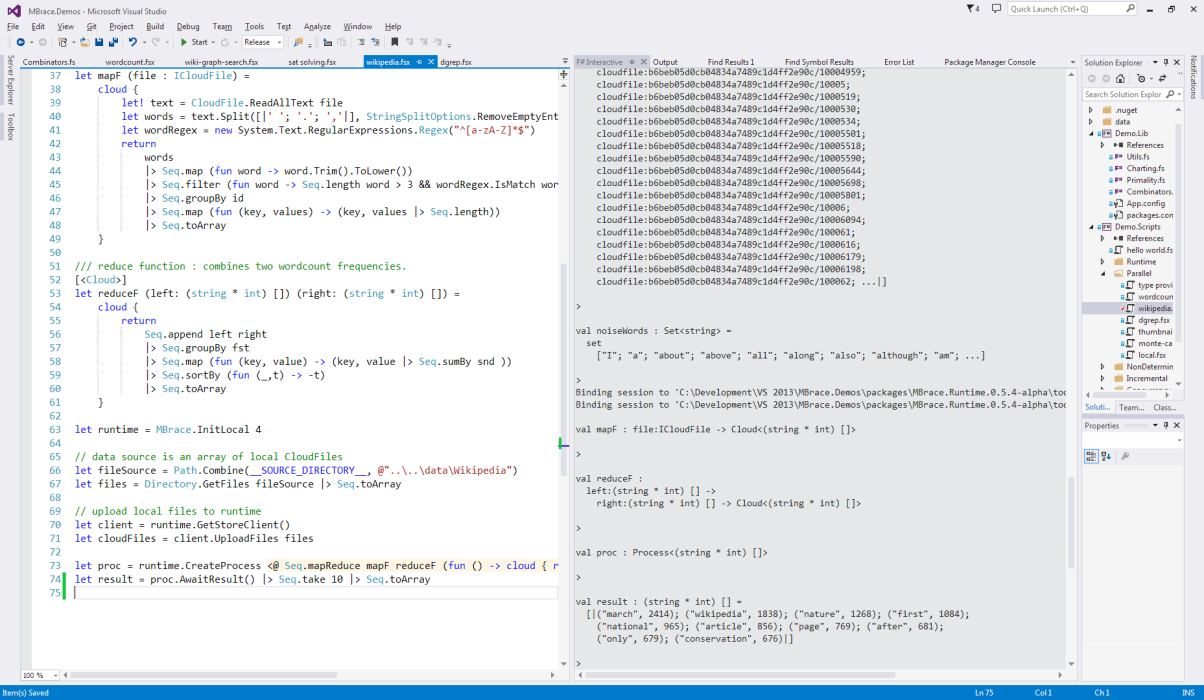
\includegraphics[width=\textwidth]{shell2.png}
\caption{The \Mbrace{} shell integrated with Visual Studio.}
\end{figure}

\subsection{The Cloud Workflow API}
\label{sec:client:workflows}

Cloud workflows can be declared using the syntax and primitives as described in section \ref{sec:workflows}.
In this segment we offer some additional information on cloud workflows that relate to the client API.

\subsubsection*{Quotations \& the Cloud Attribute}

A primary function of the \mbrace{} client is statically traversing cloud workflows 
for library dependencies, extracting metadata to be used for debugging purposes,
as well as detecting and emitting warnings for potentially invalid patterns. 
This static traversal is in part achieved through the help of \fsharp{} code quotations.
Code quotations are an excellent resource for metadata and as such, they are utilized by \mbrace{}.

As demonstrated earlier, cloud computations in \mbrace{} are initialized like so:
\begin{lstlisting}
let proc = runtime.CreateProcess <@ cloud { return 1 + 1 } @>
\end{lstlisting}
where \texttt{runtime} denotes a client object to a running \mbrace{} cluster.
A peculiar feature of this syntax is that cloud blocks are delimited by \texttt{<@} and 
\texttt{@>} symbols. These are part of the \fsharp{} language feature known as \emph{code quotations}%
\footnote{\fsharp{} Code Quotations, \samehref{http://msdn.microsoft.com/en-us/library/dd233212.aspx}}.
Any \fsharp{} expression enclosed in these symbols will yield a
typed \emph{syntax tree} of the given expression, also known as its \emph{quotation}.
The quotation expression \texttt{<@ 1 + 1 @>} has type \texttt{Expr<int>}, 
meaning that it is a syntax tree which, if evaluated, 
will yield a result of type \texttt{int}.

The \texttt{CreateProcess} method in \mbrace{} has type signature
\centertt{Expr<Cloud<\uq{}T>> -> Process<\uq{}T>}
which means that all executed cloud blocks need to be quoted.
This does not mean that all dependent workflows have to be enclosed in quotation symbols:
only the top-level expression need be so:
\begin{lstlisting}
[<Cloud>]
let test () = cloud { return 1 }

runtime.Run <@ test () @>
\end{lstlisting}

Despite this, all nested calls to cloud workflows should be affixed with a \texttt{[<Cloud>]}
attribute. Failing to do so will result in warning messages being raised.
The \texttt{CloudAttribute} is just an abbreviation of the \texttt{ReflectedDefinitionAttribute}%
\footnote{See, \samehref{http://msdn.microsoft.com/en-us/library/ee353643.aspx}}
provided by \fsharp{}. Adding this to a declaration makes the \fsharp{} compiler generate a 
reflected quotation to the tagged code.

It should be noted that the \texttt{Cloud} attribute is not needed for \fsharp{} declarations 
that are not cloud workflows. For example, the following code is perfectly valid:
\begin{lstlisting}
let f x = x + 1

[<Cloud>]
let g () = cloud { return f 41 }
\end{lstlisting}

\subsubsection*{The \TitularMbrace{} Shell}

The \mbrace{} shell is a cloud development facility that is based on \fsharp{} interactive.
It permits ad hoc declaration, deployment and debugging of cloud workflows directly from the REPL. 
This is made possible through a Vagrant%
\footnote{\samehref{http://nessos.github.io/Vagrant}}
, a general purpose code distribution library for \dotnet{}.
\begin{verbatim}
   > [<Cloud>] let f x = cloud { return 2 * x } ;;

   val f : unit -> Cloud<int>

   > runtime.Run <@ f 21 @> ;;
   compiling interactions to assembly... 
   uploading assemblies to runtime... 
   val it : int = 42
   >
\end{verbatim}
The \mbrace{} shell is also capable of including custom types to computations.
\begin{verbatim}
   > type Container = Content of int ;;

   type Container = | Content of int

   > match runtime.Run <@ cloud { return Content 42 } @> with
   | Content 42 -> printfn "success"
   | _ -> printfn "failure" ;;
   compiling interactions to assembly... 
   uploading assemblies to runtime... 
   success
   val it : unit = ()
\end{verbatim}


\subsubsection*{Value Declarations \& Side Effects}

We now describe a technical issue that is related to the distributed nature of cloud computation.
Consider a library that includes the following code:
\begin{lstlisting}
let data = System.IO.File.ReadAllBytes "/Users/eirik/Desktop/1.dat"

[<Cloud>]
let getSize () = cloud { return data.Length }

let run () = runtime.Run <@ getSize () @>
\end{lstlisting}
One might hold the expectation that the \texttt{data} will be read at the client side,
with the cloud workflow segment of the computation taking place at the runtime.
This is not the case however: in fact, \texttt{data} will be read \emph{in every}
node of the runtime separately. This can lead to unanticipated errors, in this case
having to do with the fact that \texttt{1.dat} does only exist in the client computer.

The problem occurs because \texttt{data} is a library artifact, not something
that relates to client-side execution explicitly. In the \fsharp{} compiler in particular,
let-bound values are initialized using underlying static constructors, which are triggered
whenever the parent library gets used, be it the client or the runtime.
Since \mbrace{} distributes depended libraries to all worker nodes, type initialization 
side-effects are going to be triggered everywhere.

Value initialization issues can be typically resolved by demoting such values from top-level
declarations:
\begin{lstlisting}
[<Cloud>]
let getSize (data : byte []) = cloud { return data.Length }

let run () = 
	let data = System.IO.File.ReadAllBytes "/Users/eirik/Desktop/1.dat" in
	runtime.Run <@ getSize data  @>
\end{lstlisting}

An important exception to the above behaviour is the \mbrace{} shell. The shell has the 
important property that both compilation and execution take place in the same process. 
Moreover, patterns like the one described above are very common in repl environments.
This has allowed us overcome the above problem for certain data types using a technique
that involves code erasure of value initializers in the assemblies compiled by the shell.

\subsubsection*{Non-Serializable Objects}

\noindent Consider the following snippet:
\begin{lstlisting}
cloud {
	let http = new System.Net.WebClient()
	let download url = cloud { return http.DownloadString url }
	return! 
		Cloud.Parallel <| 
			Array.map download 
				[| "http://www.m-brace.net" ; "http://www.nessos.gr" |]
}
\end{lstlisting}
This workflow is clearly wrong, since it demands the distribution of an evidently
nondistributable local resource, an instance of \texttt{WebClient}.
In fact, attempting to submit this workflow to a runtime for execution will result in
an error, since the client will detect that it uses instances of non-serializable 
types.

Cloud workflows do not support environments with non-serializable objects,
and for good reason. So how does one integrate code that utilizes types such
as file streams, web sockets, etc?
%
The answer is to encapsulate locally scoped objects in an execution context
that enforces local semantics. This can be done using native \fsharp{} code:
\begin{lstlisting}
let download (url : string) =
	use http = new System.Net.WebClient()
	http.DownloadString url

cloud {
	return! Cloud.Parallel <|
		Array.map (fun u -> cloud { return download u })
			[| "http://www.m-brace.net" ; "http://www.nessos.gr" |]
}
\end{lstlisting}
or by embedding \texttt{async} workflows:
\begin{lstlisting}
let downloadAsync (url : string) = async {
	use http = new System.Net.WebClient()
	return! http.DownloadStringAsync url
}

cloud {
	return! Cloud.Parallel <|
		Array.map (Cloud.OfAsync << downloadAsync)
			[| "http://www.m-brace.net" ; "http://www.nessos.gr" |]
} 
\end{lstlisting}

The above coding style reflects the operation philosophy of \mbrace:
cloud workflows ought to be restricted to the orchestration of distribution patterns, 
whereas computation taking place within the context of a single worker 
had preferably be elaborated in native \dotnet{} or async workflows.

\subsubsection*{Local Execution}

In absence of a runtime, cloud workflows can be executed locally using the method
%
\centertt{MBrace.RunLocal : Cloud<\uq{}T> -> \uq{}T}
%
This will run the workflow in a local interpreter with execution semantics that resemble
but do not coincide with those of Async: while distribution does occur through thread 
concurrency, it differs in certain subtleties that are introduced artificially so that 
the execution model of the \mbrace{} runtime is more closely emulated.
For more information, please refer to the \href{peculiarities}{``Semantic Peculiarities''}
segment of section \ref{sec:workflows}.

\subsection{Store Providers}

Every \mbrace{} runtime requires a storage backend in order for it to function.
This enables distributed storage primitives like cloud refs and cloud files and
is used by internally the runtime for logging purposes.
The \mbrace{} runtime does not provide its own distributed storage implementation, 
rather it relies on pluggable storage providers which can be user defined.
\begin{lstlisting}
open Nessos.MBrace.Store

let fsStore = FileSystemStore.Create(@"\\FileServer\path\to\mbrace")
let sqlStore = SqlServerStore.Create(connectionString = "connectionString")

open Nessos.MBrace.Azure

let azureStore = AzureStore.Create(accountName = "name", accountKey = "key")
\end{lstlisting}
The default store implementation of a client session can be specified by setting
\begin{lstlisting}
MBraceSettings.DefaultStore <- azureStore
\end{lstlisting}
User-defined storage providers can be created by implementing the \texttt{ICloudStore} interface. 
For more information, please consult the \mbrace{} API reference.

\subsection{Managing \TitularMbrace{} Runtimes}

The \mbrace{} runtime is a cluster of connected computers capable of orchestrating the execution
of cloud workflows. Every computer participating in an \mbrace{} runtime is known as an \mbrace{}
\emph{node}. In this section we offer an overview of how the \mbrace{} client stack can be
used to initialize, manage and monitor remote \mbrace{} runtimes.

\subsubsection*{The MBraceNode Type}

An \mbrace{} \emph{node} represents any physical machine that runs the \emph{\mbrace{}} daemon, 
the server-side component of the framework. Every \mbrace{} daemon accepts connections from a predetermined 
\texttt{tcp} port on the host. \Mbrace{} nodes are identifiable by the uri format
\centertt{mbrace://hostname:port/}
The \mbrace{} client can connect to a remote node by calling
\begin{lstlisting}
let node = Node.Connect("mbrace://hostname:2675")
\end{lstlisting}
or equivalently,
\begin{lstlisting}
let node = Node.Connect("hostname", 2675)
\end{lstlisting}
This will initialize an object of type \texttt{MBraceNode}. This object acts as a handle
to the remote node. It can be used to perform a variety of operations like
\begin{lstlisting}
node.Ping() // ping the node, returning the number of milliseconds taken
\end{lstlisting}
or
\begin{lstlisting}
node.IsActive : bool
\end{lstlisting}
which is a property indicating whether the node is part of an existing \mbrace{} cluster.

Every \mbrace{} daemon writes to a log of its own. \Mbrace{} node logs can accessed remotely
from the client either in the form of a dump
\begin{lstlisting}
node.ShowSystemLogs()
\end{lstlisting}
or in a structured format that can be used to perform local queries:
\begin{lstlisting}
node.GetSystemLogs() 
|> Seq.filter (fun entry -> DateTime.Now - entry.Date < TimeSpan.FromDays 1.)
\end{lstlisting}

\subsubsection*{The MBraceRuntime Type}

An \mbrace{} runtime can be \emph{booted} once access to a collection of at least two nodes,
all running within the same subnet, has been established. This can be done like so:
\begin{lstlisting}
let nodes : Node list = [ node1 ; node2 ; node3 ]

let runtime = MBraceRuntime.Boot(nodes, store = azureStore)
\end{lstlisting}
This will initialize an \mbrace{} cluster that connects to a Windows Azure store endpoint.
Once boot is completed, a handle of type \texttt{MbraceRuntime} will be returned.
If no store is specified explicitly, the \texttt{MBraceSettings.DefaultStore} will be used.
%
To connect to an already booted \mbrace{} runtime, one needs simply write
\begin{lstlisting}
let runtime = MBraceRuntime.Connect("mbrace://host:port/")
\end{lstlisting}
wherein the supplied uri can point to any of the constituent worker nodes.

The client stack provides a facility for instantaneously spawning local runtimes:
\begin{lstlisting}
let runtime = MBraceRuntime.InitLocal(totalNodes = 4, background = true)
\end{lstlisting}
This will initiate a runtime of four local nodes that execute in the background.
The feature is particularly useful for quick deployments of distributed code under development.

The \texttt{MBraceRuntime} object serves as the entry point for any kind of client interactions 
with the cluster. For instance, the property
\begin{lstlisting}
runtime.Nodes : Node list
\end{lstlisting}
returns the list of all nodes that constitute the cluster.
In the \mbrace{} shell, calling
\begin{lstlisting}
runtime.ShowRuntimeInfo()
\end{lstlisting}
prints a detailed description of the cluster to the terminal.
\begin{verbatim}
   {m}brace runtime information (active)                                               

   Host           Port  Role        Location          Connection String            
   ----           ----  ----        --------          -----------------            
   grothendieck  38857  Master      Local (Pid 3008)  mbrace://grothendieck:38857/ 
   grothendieck  38873  Alt Master  Local (Pid 3616)  mbrace://grothendieck:38873/ 
   grothendieck  38865  Alt Master  Local (Pid 4952)  mbrace://grothendieck:38865/ 
\end{verbatim}
The state of the runtime can be reset or stopped at any point by calling the following methods:
\begin{lstlisting}
runtime.Shutdown() // stops the runtime
runtime.Reboot() // resets the state of the runtime
runtime.Kill() // violently kills all node processes in the runtime
\end{lstlisting}

\subsection{Managing Cloud Processes}

A \emph{cloud process} is a currently executing or completed cloud computation in the context
of a specific \mbrace{} runtime. In any given runtime, cloud processes can be initialized,
monitored for progress, or cancelled; completed cloud processes can be queried for their results
and symbolic stack traces can be fetched for failed executions.

Cloud processes form a fundamental organizational unit for the \mbrace{} runtime:
conceptually, if one is to think of \mbrace{} as an operating system for the cloud,
then cloud processes form its units of distributed execution;
every cloud process spawns its own set of scheduler and workers;
the \mbrace{} runtime enforces a regime of \emph{process isolation},
which means that each cloud process will run in a distinct instance of the CLR in the context
of each worker node.

Given a \emph{runtime} object, a cloud process can be initialized like so:
\begin{lstlisting}
let proc = runtime.CreateProcess <@ cloud { return 1 + 1 } @>
\end{lstlisting}
This will submit the workflow to the runtime for execution and return with a process handle of
type \texttt{Process<int>}. Various useful properties can be used to query the status of the
cloud computation at any time. For instance,
\begin{lstlisting}
proc.Result // Pending, Value, user Exception or system Fault
proc.ProcessId // the cloud process id
proc.InitTime // returns a System.DateTime on execution start
proc.ExecutionTime // returns a System.TimeSpan on execution time
proc.GetLogs() // get user logs for cloud process
\end{lstlisting}
If running in the \mbrace{} shell, typing the command
\begin{verbatim}
   > proc.ShowInfo() ;;
\end{verbatim}
will print information like the following
\begin{verbatim}
 Name       Process Id  Status   #Workers  #Tasks  Start Time         Result Type       
 ----       ----------  ------   --------  ------  ----------         -----------       
 mapReduce        6674  Running         2       2  30/7/2013 4:08:21  (string * int) [] 
\end{verbatim}
Similar to \texttt{CreateProcess} is the \texttt{Run} method:
\begin{lstlisting}
let result : int = runtime.Run <@ cloud { return 1 + 1 } @>
\end{lstlisting}
This is a blocking version of \texttt{CreateProcess} that is equivalent to the statement below:
\begin{lstlisting}
let proc = runtime.CreateProcess <@ cloud { return 1 + 1 } @> in
proc.AwaitResult()
\end{lstlisting}
%
The \texttt{AwaitResult} method also comes in an asynchronous flavour
\begin{lstlisting}
let task : Task<int> = proc.AwaitResultAsync() |> Async.StartAsTask
\end{lstlisting}
%
A list of all executing cloud processes in a given runtime can be obtained as follows:
\begin{lstlisting}
let procs : Process list = runtime.GetAllProcesses()
\end{lstlisting}
This will return a list of \emph{untyped} cloud process handles.
If running in the \mbrace{} Shell, process information can be printed to the buffer like so:
\begin{verbatim}
   > runtime.ShowProcessInfo() ;;
\end{verbatim}
Given a cloud process id, one can receive the corresponding handle object like so:
\begin{lstlisting}
let proc : Process = runtime.GetProcess 1131
let proc' : Process<string> = runtime.GetProcess<string> 119
\end{lstlisting}
Finally, an executing cloud process can be cancelled with the following method
\begin{lstlisting}
proc.Kill()
\end{lstlisting}

\subsection{\TitularMbrace{} Client Settings}

Certain aspects of the \mbrace{} client can be configured by the user.
This is done through the \texttt{MBraceSettings} fa\c{c}ade that contains an
assortment of property getters and setters:
\begin{itemize}
\item The \texttt{MBraceSettings.DefaultStore} gets or sets the default store provider
used by this client session. Serves as the default store provider used in newly booted
nodes and runtimes. Please refer to the runtime section of this document.
\item The \texttt{MBraceSettings.MBracedExecutablePath} gets or sets the path to the
local \texttt{mbraced} executable. This is used by the client to spawn local instances
of \mbrace{} nodes.
\item The \texttt{MBraceSettings.AssemblyCachePath} gets or sets the local system 
path in which the client caches user generated assemblies.
\item The \texttt{MBraceSettings.LocalCachePath} gets or sets the local system path
in which items like cloud refs or cloud files are cached with the client.
\end{itemize}
%
%
%	Section 3: The Mbrace runtime
%

\section{The \TitularMbrace{} Distributed Runtime}
\label{sec:runtime}

The \mbrace{} runtime is the execution environment of the \mbrace{} framework
that implements the execution semantics of cloud workflows and cloud data
as described previously. A typical \mbrace{} runtime instance comprises
multiple nodes forming a cluster. The runtime is responsible for executing cloud
workflows, managing and monitoring the nodes and resources within a cluster,
elasticity, fault tolerance and integration with distributed storage providers.

From a user's perspective the \mbrace{} runtime provides an abstraction over a
cluster analogous to that of an operating system over hardware. A cloud
workflow, representing a deferred computation as described earlier, along with
any code and dependencies effectively forms the cloud program executable by the
runtime, of which an executing instance is a \emph{cloud process}. Multiple
cloud processes are executed concurrently and in isolation in the much the same
sense as in traditional multi-process operating systems. The runtime monitors
and manages the computational and data resources available within the cluster,
which are allocated between cloud processes based on load and runtime
statistics.
%
\begin{figure}[ht]
\label{runtime-figure}
\centering
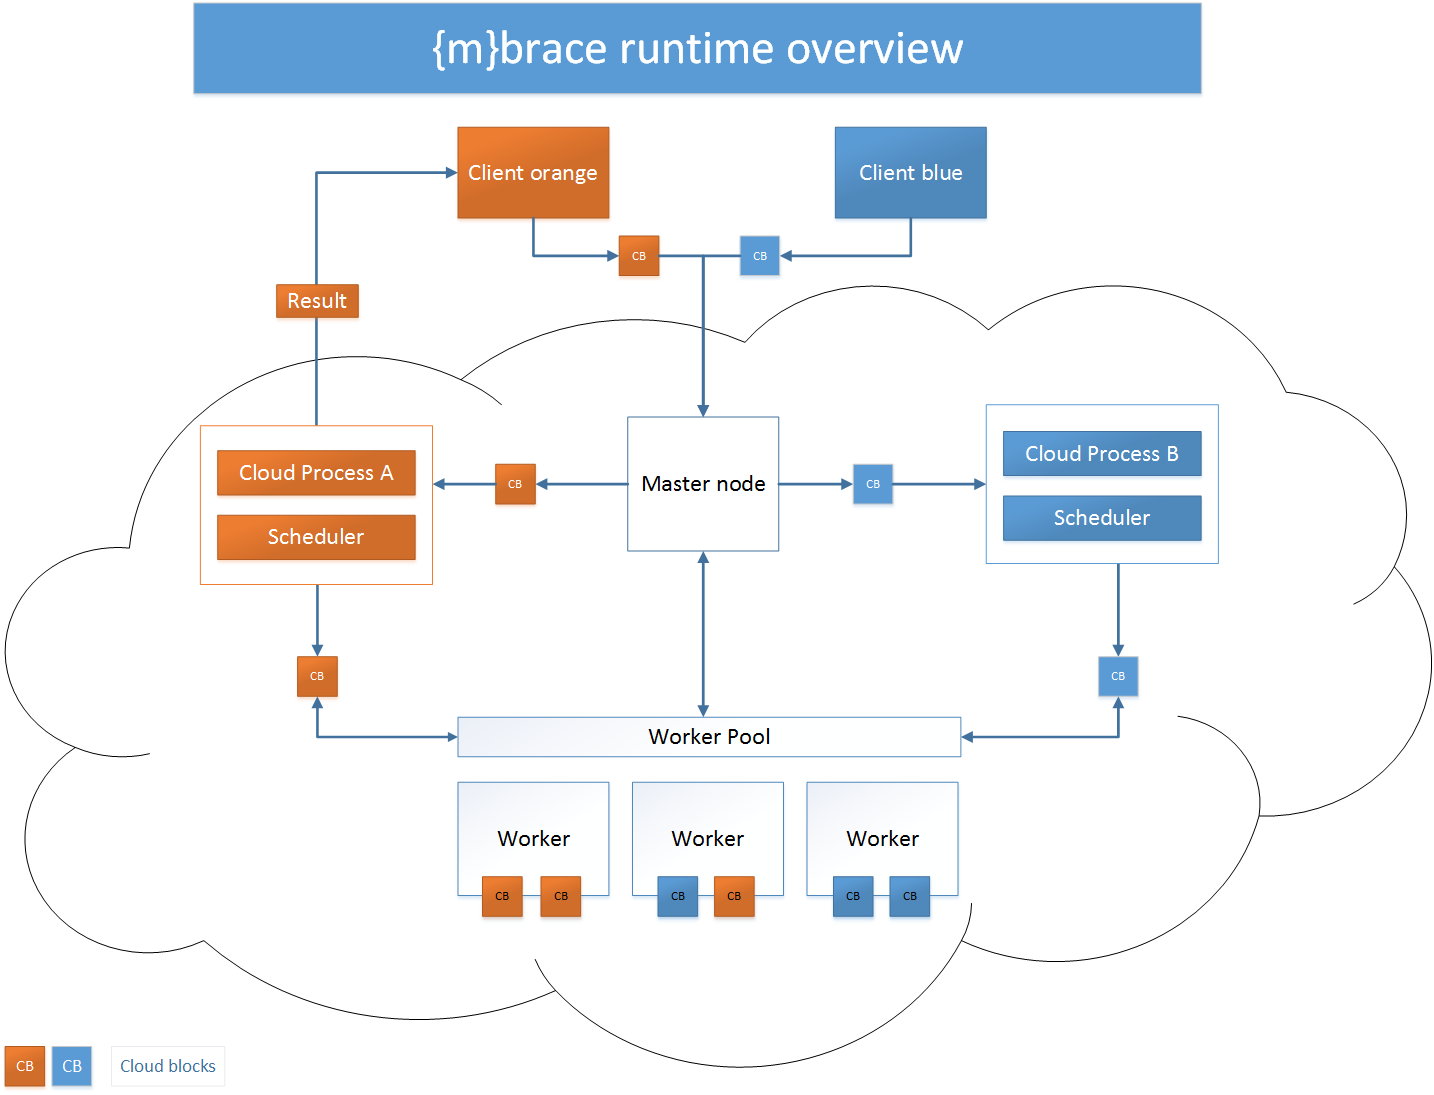
\includegraphics[width=0.8\textwidth]{runtime.png}
\caption{Architectural overview of the \mbrace{} runtime.}
\end{figure}

In figure \ref{runtime-figure} we give an architectural overview of a \mbrace{}
cluster instance. Each cluster instance has a unique \emph{master node} which is
responsible for monitoring the health of the nodes participating in the cluster
as well as gathering other runtime statics, such as CPU and network loads. All
other nodes are slave nodes. A subset of slave nodes are \emph{alternative
  masters}. Alternative master nodes replicate the master node's state. In the
event of a master node failure, a new master node will be selected from the
available alternatives while a slave node will be added to the alternative set.

The execution of a cloud process employs a \emph{scheduler-worker} scheme. One
node is selected to be the process scheduler with the rest being worker
nodes. The scheduler unfolds the cloud workflow in execution and allocates
pending jobs to available workers. Scheduling is load balanced taking into
account relevant runtime statics such as CPU and network load of the available
workers. The scheduler maintains state tracking the job allocation, which is
replicated between a subset of the available worker nodes. In the event of a
worker node failure this allows the scheduler to re-schedule any lost jobs,
while in the event of the scheduler node failure a new scheduler is selected
from the available worker nodes and its state is re-applied.

Cluster nodes are shared between concurrently executing cloud
processes. However, the runtime enforces an \emph{isolation} policy where each
cloud process is allocated a distinct CLI instance in each node. The set of all
CLI instances allocated to a cloud process is the unit isolation and is called a
\emph{process domain}. Each cloud process inhibits a distinct process
domain. Thus a single cluster node may host multiple CLI scheduler and worker
instances from different cloud processes. This enables a more robust runtime as
local process failures are isolated and leads to more efficient memory
management as each CLI instance has its own garbage collector. Note that each
cloud process is allocated its own scheduler offering a further level of
isolation in terms of scheduling load. Again, allocating schedulers to cloud
processes is balanced between the available nodes.

Finally, the \mbrace{} runtime offers pluggable support for a range of
distributed store providers. Storage providers are essential for a runtime to
function, since they are used for internal caching and make possible the
definition of cloud refs. \mbrace{} comes with support for FileSystem, SQL and
Azure storage providers, while providing user-defined custom implementations is
also possible.

\subsection{The \TitularMbrace{} Daemon}

As mentioned earlier, the \mbrace{} daemon is the server-side application that
contains a machine-wide instance of the \mbrace{} framework. It is initialized by
running the \texttt{mbraced.exe} executable, typically found in the \texttt{tools}
folder of the \texttt{MBrace.Runtime} nuget package. For instance, the command
\begin{verbatim}
   $ mbraced.exe --hostname 127.0.0.1 --primary-port 2675 --detach
\end{verbatim}
will instantiate a background \texttt{mbraced} process that listens on
the loopback interface at port 2675.

\subsubsection*{Configuring the \TitularMbrace{} Daemon}

The \mbrace{} daemon comes with a range of configuration options.
These parameters can either be read from the \texttt{mbraced} configuration file, 
or passed as command line arguments, in that evaluation order.
Command line parameters override those provided by the configuration file.

As is common in \dotnet{} applications, \texttt{mbraced} comes with an xml
configuration file, namely \texttt{mbraced.exe.config} found in the same location 
as the executable. Configuration for \texttt{mbraced} is written in the 
\texttt{AppSettings} section of the xml document that follows a key-value 
schema:
\begin{lstlisting}[language=Xml]
<?xml version="1.0" encoding="utf-8"?>
<configuration>
  <appSettings>
    <add key="hostname" value="grothendieck.nessos"/>
    <add key="primary port" value="2675"/>
    <add key="worker port range" value="30000, 30042"/>
    <add key="working directory" value="/var/mbraced/"/>
    <add key="log file" value="mbrace-log.txt"/>
    <!-- specify loglevel: info 0, warning 1, error 2-->
    <add key="log level" value="0"/>
    <!-- permitted operation modes; None: 0, Slave: 1, Master: 2, All: 3 -->
    <add key="permissions" value="3" />
    <!-- executable name of mbrace child process -->
    <add key="mbrace processdomain executable" value="mbrace.worker.exe"/>
  </appSettings>
</configuration>
\end{lstlisting}
The full range of command line parameters for \texttt{mbraced} can be viewed by typing
\begin{verbatim}
   $ mbraced.exe --help
\end{verbatim}
%
We now give a brief description of the configuration parameters offered by the daemon:
\begin{description}[style=unboxed, font=\sffamily]
\item[Hostname] The ip address or host name that the daemon listens to.
The hostname must be resolvable in the context of the entire \mbrace{} cluster.
Each instance of \texttt{mbraced} can only have one hostname specified.
\item[Primary Port] The tcp port that the local cluster supervisor listens to.
\item[Worker Port Range] A range or collection of tcp ports that can be assigned
to worker processes spawned by the local cluster supervisor.
\item[Working Directory] The local directory in which all local caching is performed.
Write permissions are required for the daemon process.
\item[Log File] Specifies the path to the log file. If relative, it is resolved with
respect to the working directory.
\item[Log Level] Specifies the log level: 0 for info, 1 for warnings, 2 for errors.
\item[ProcessDomain Executable] The location of the worker process executable.
Relative paths evaluated with respect to the main \texttt{mbraced.exe} path.
\end{description}

\subsubsection*{Deploying the \TitularMbrace{} Daemon}

Once the configuration file for \texttt{mbraced} has been set up as desired,
deploying an instance from the command line is as simple as typing
\begin{verbatim}
    $ mbraced --detach
\end{verbatim}
The \mbrace{} framework also comes with the \texttt{mbracectl} command line tool
that can be used to track deployment state. Initiating a session can be done like so:
\begin{verbatim}
    $ mbracectl start
\end{verbatim}
This will initialize a background instance with settings read from the \texttt{mbraced}
configuration file. Session state can be queried by entering
\begin{verbatim}
    $ mbracectl status
\end{verbatim}
Finally, a session can be ended by typing
\begin{verbatim}
    $ mbracectl stop
\end{verbatim}
\texttt{mbracectl} can also be used to initiate multiple instances on the local machine
\begin{verbatim}
    $ mbracectl start --nodes 16 --spawn-window
\end{verbatim}
that can even be booted in a local cluster
\begin{verbatim}
    $ mbracectl start --nodes 3 --boot
\end{verbatim}

The \mbrace{} runtime package also comes bundled with a windows service.
Initiating \texttt{mbraced} as a service will spawn a background instance
with settings read from the xml configuration file.

Once the required \texttt{mbraced} instances have been deployed as desired,
they can be reached from the client API as seen in section \ref{sec:client}
using the \texttt{mbrace} connection string.

%
\appendix
%
%
%	Appendix
%

\section*{Appendix}

\subsection*{Future Work}

\Mbrace{} is a large project that faces multiple technical challenges. As such,
it remains (as of the private alpha release) a work in progress with many important
features still under development. In this section we discuss some of the features
which we consider to be important milestones in the future of the \mbrace{} project.

\subsubsection*{\csharp{}-LINQ support}
CloudLinq% 
\footnote{\samehref{https://github.com/nessos/CloudLinq}}
is a satellite project for \mbrace{} aiming at providing an idiomatic 
API for the immensely popular \csharp{} language in the
form of a LINQ provider%
\footnote{\samehref{http://msdn.microsoft.com/en-us/library/vstudio/bb397926.aspx}}
for data parallelism. This would allow building cloud workflows using simple
LINQ-style queries:
\begin{lstlisting}[language=CSharp]
var result =  from c in Customers.AsCloudQueryExpr()
			  where c.City == "Athens"
			  orderby c.Name
			  select c.Name, c.City
\end{lstlisting}
CloudLinq can achieve excellent performance by taking advantage of LinqOptimizer%
\footnote{\samehref{https://github.com/nessos/LinqOptimizer}}
which is an optimizer for Linq and compiles declarative queries into fast imperative code. Another interesting direction is the combination
of CloudLinq with GpuLinq%
\footnote{\samehref{https://github.com/nessos/GpuLinq}}
in order to compile queries to OpenCL kernel code for fast execution on GPU powered cloud instances.

\subsubsection*{Mono Support}

The Mono project%
\footnote{The Mono project, \samehref{http://www.mono-project.com/}.}
is a popular open source implementation of Microsoft's \dotnet{} framework.
The Mono framework is in the unique position of offering a truly cross-platform
\dotnet{} development experience as it supports most major operating systems,
including Linux and Mac OS X.

Just like the \fsharp{} language itself, we believe that a big part of \mbrace{}'s 
future lies with Mono and the open source community in general. Providing support
for the Mono framework is strategically important since it opens up the market
to diverse developer cultures and data center infrastructures.


% TODO: fill out the following sections

%\subsection*{Web UI}

%\subsection*{Internals Discussion}
%
%\subsubsection*{The Distributed Actor Framework}
%
%\subsubsection*{Serialization}
%
%\subsubsection*{The Monadic Trampoline}

%
%	Bibliography secion
%	TODO: bibtex
%

\begin{thebibliography}{9}

	\bibitem{map-reduce} J. Dean, S. Ghemawat. 
		\emph{MapReduce: Simplified Data Processing on Large Clusters}, \\
		OSDI '04, p. 137--150.
		\samehref{http://www.usenix.org/events/osdi04/tech/dean.html}

	\bibitem{cloud-haskell} J. Epstein, A.P. Black, S.P. Jones.
		\emph{Towards Haskell in the Cloud},\\
		\samehref{http://research.microsoft.com/en-us/um/people/simonpj/papers/parallel/remote.pdf}
		
	\bibitem{HdpH} P. Maier and P. Trinder.
		\emph{Implementing a High-level Distributed-Memory Parallel Haskell in Haskell},\\
		\samehref{http://www.macs.hw.ac.uk/~trinder/papers/HdpH.pdf}
		
	\bibitem{par-monad} S. Marlow, R. Newton, S.P. Jones.
		\emph{A monad for deterministic parallelism},\\
		\samehref{http://research.microsoft.com/en-us/um/people/simonpj/papers/parallel/monad-par.pdf}
		
	\bibitem{ShmStreaming} L. Lai, J. Zhou, L. Zheng, H. Li, Y. Lu, F. Tang, M. Guo.
		\emph{ShmStreaming: A Shared Memory Approach for Improving Hadoop Streaming Performance},\\
		\samehref{http://www.computer.org/csdl/proceedings/aina/2013/4953/00/4953a137-abs.html}
			
	\bibitem{HaLoop} Y. Bu, B. Howe, M. Balazinska, M. D. Ernst.
		\emph{HaLoop: Efficient Iterative Data Processing on Large Clusters},\\
		\samehref{http://dl.acm.org/citation.cfm?id=1920881}
		
	\bibitem{IncMR} C. Yan, X. Yang, Z. Yu, M. Li, X. Li.
		\emph{IncMR: Incremental Data Processing based on MapReduce},\\
		\samehref{http://www.bibsonomy.org/bibtex/29cb17af55bcdf7a99bfd4e0e62bccf73/dblp}
	
	\bibitem{fsharp-compexpr} T. Petricek, D. Syme.
		\emph{Syntax Matters: Writing abstract computations in \fsharp},\\
		Pre-proceedings of TFP, 2012.\\
		\href{http://www.cl.cam.ac.uk/~tp322/drafts/notations.pdf}
			{\texttt{http://www.cl.cam.ac.uk/{\textasciitilde}tp322/drafts/notations.pdf}}

	\bibitem{fsharp-async} D. Syme, T. Petricek T, D. Lomov.
		\emph{The \fsharp{} Asynchronous Programming Model}. \\ 
		\samehref{http://research.microsoft.com/apps/pubs/default.aspx?id=147194}.
		
	\bibitem{data-types-ala-carte} 
		W. Swierstra. \emph{Data types \`{a} la carte}, Journal of Functional Programming, \\ 	   
		Cambridge University Press, 2008. \\
		\href{http://www.cs.ru.nl/~W.Swierstra/Publications/DataTypesALaCarte.pdf}
			{\texttt{http://www.cs.ru.nl/{\textasciitilde}W.Swierstra/%
						Publications/DataTypesALaCarte.pdf}}
		
	\bibitem{scala-trampolines}
		R.O. Bjarnarson. \emph{Stackless Scala With Free Monads}. Scala Days 2012.\\
		\samehref{http://blog.higher-order.com/assets/trampolines.pdf}

\end{thebibliography}

\end{document}

%%% Local Variables: 
%%% mode: latex
%%% TeX-master: "mbrace"
%%% End: 
